\documentclass[a4paper,twoside,15pt]{book}
\usepackage[utf8]{inputenc}
\oddsidemargin=1cm
\evensidemargin=1cm
\addtolength{\textwidth}{1in}
\addtolength{\voffset}{-5pt}

\title{Moravia Microsystems - Corporate Coding Convention}
\author{Martin Ošmera <martin.osmera@moravia-microsystems.com.com>}

\newcommand{\mysubject}{Moravia Microsystems, the Corporate Coding Convention.}
\newcommand{\mykeywords}{Moravia Microsystems}

\usepackage[T1]{fontenc}
\usepackage{float}
\usepackage{graphicx}
\usepackage{fancyhdr}
\usepackage{longtable}
\usepackage[usenames,dvipsnames]{color}
\usepackage{pifont}
\usepackage{wrapfig}
\usepackage[footnotesize,bf]{caption}
\usepackage[pdftex,colorlinks=true,linkcolor=blue,urlcolor=blue,pdftitle={\title{}},pdfauthor={\author{}},pdfsubject={\mysubject{}},pdfkeywords={\mykeywords{}},bookmarksopen=false,pdfpagemode=None]{hyperref}
\usepackage{eurosans}
\usepackage{colortbl}

\floatstyle{ruled}
\newfloat{code}{thp}{lop}
\floatname{code}{Code}

\renewcommand{\chaptermark}[1]{\markboth{\thechapter.\ \MakeUppercase{#1}}{}}
\renewcommand{\sectionmark}[1]{\markright{\thesection\ #1}}

\newcommand{\menuitem}[1]{\texttt{#1}}
\newcommand{\fileextension}[1]{\texttt{#1}}
\newcommand{\mysmallfont}{\fontsize{8pt}{10pt} \selectfont{}}
\newcommand{\uC}{$\mu$C }

\pdfadjustspacing=1
\raggedbottom

\pagestyle{fancy}
\fancyhf{}
\fancyhead[EL,OR]{\bfseries\thepage}
\fancyhead[LO]{\bfseries\rightmark}
\fancyhead[RE]{\bfseries\leftmark}

\fancypagestyle{plain}{
    \fancyhead{}
    \fancyhead[EL,OR]{\bfseries\thepage}
    \renewcommand{\headrulewidth}{0pt}
}

% define colors for syntax highlight
\definecolor{highlight_c_keyword}{rgb}{0.0, 0.0, 0.866}
\definecolor{highlight_c_data_type}{rgb}{0.0, 0.8, 0.0}
\definecolor{highlight_c_dec}{rgb}{0.0, 0.0, 1.0}
\definecolor{highlight_c_hex}{rgb}{0.533, 0.0, 1.0}
\definecolor{highlight_c_comment}{rgb}{0.533, 0.533, 0.533}
\definecolor{highlight_c_symbol}{rgb}{1.0, 0.0, 0.0}
\definecolor{highlight_c_bracket}{rgb}{0.933, 0.4, 0.0}
\definecolor{highlight_c_preprocessor}{rgb}{0.0, 0.533, 0.0}
\definecolor{highlight_c_directive}{rgb}{0.333, 0.533, 0.0}
\definecolor{highlight_c_prep_lib}{rgb}{0.533, 0.333, 0.0}
\definecolor{highlight_normal}{rgb}{0.0, 0.0, 0.0}
\definecolor{highlight_c_dox_comment}{rgb}{0.266, 0.266, 1.0}
\definecolor{highlight_c_dox_tag}{rgb}{0.666, 0.0, 0.866}
\definecolor{highlight_c_dox_word}{rgb}{0.0, 0.533, 1.0}
\definecolor{highlight_c_dox_name}{rgb}{1.0, 0.0, 0.0}

\begin{document}

\begin{titlepage}
    \begin{figure}[ht!]
        \centering{}
        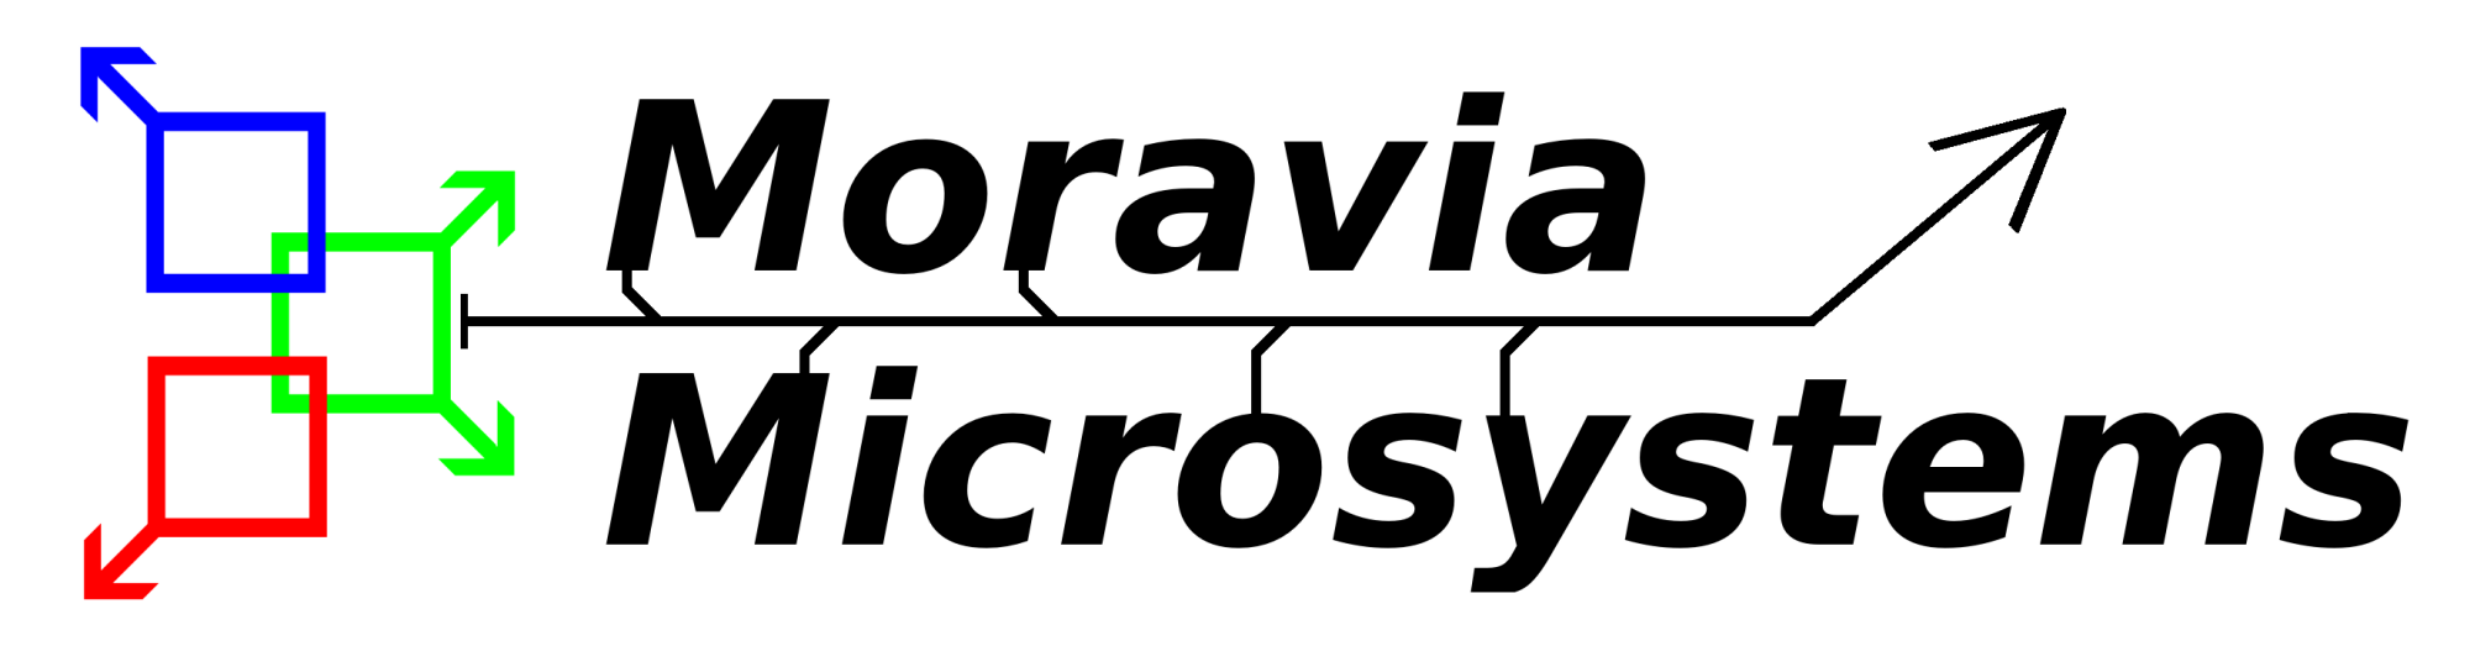
\includegraphics[width=.9\textwidth]{Moravia_Microsystems.png}
        \caption{\textit{Moravia Microsystems, s.r.o.}}
    \end{figure}
    \begin{center}
        \fontsize{35.83pt}{60pt} \selectfont{}
        \textbf{Coding Convention}
        \\[2cm]
        \fontsize{25pt}{30pt} \selectfont{}
        Corporate coding convention\\
        guildelines for C++ and C.
        \\[1cm]
        \fontsize{15pt}{19pt} \selectfont{}
        Martin Ošmera\\
        Brno, 2013
    \end{center}
\end{titlepage}

Copyright Information:
\\
Copyright \copyright{} 2013, 2014 Moravia Microsystems, s.r.o. All rights reserved.\\
Brno, Czech Republic, European Union.
\\
This document is protected by copyright. No part of this document may be reproduced in any form by any means
without prior written authorization of Moravia Microsystems, s.r.o, if any.

\tableofcontents

\chapter{Importance of a code convention}
    First of all it is important to keep in mind that this convention is not supposed to create a set of unnecessary and unproductive rules to poison your work; instead in case you are sure that your work goes better with another coding style, go ahead but please at least read this paragraph till end. Coding convention is something you probably get used to, sooner or later, and it contributes in creating unified working environment where you always know what to expect. Also it helps to write code which is relatively easily readable for someone who is familiar with the applied convention.

    \paragraph{}
    Code conventions are important to programmers for a number of reasons:
    \begin{itemize}
        \item About 80\% of the lifetime cost of a piece of software goes to maintenance.
        \item Hardly any software is maintained for its whole life by the original author.
        \item Code conventions improve the readability of the software, allowing engineers to understand new code more quickly and thoroughly.
        \item If you ship your source code as a product, you need to make sure it is as well packaged and clean as any other product you create.
    \end{itemize}

\chapter{Detailed specification}
    \section{General}
        \subsection{File names}
            \paragraph{}
            All header files should contain exactly one class, or struct, or namespace in the root namespace; name of this data type or namespace has to be the same as name of the file itself; this convention has already been already adopted by the Java programming language. Other classes, structs, and namespaces should be declared/defined only withing this one ``main'' class, struct, or namespace. Unless it is necessary, the header file should not contain any declarations outside the class, struct, or namespace.

            \paragraph{}
            Use the following file suffixes:\\
            \begin{table}[h!]
                \begin{tabular}{l|l}
                    \textbf{File Type}  & \textbf{Suffix} \\\hline
                    C/C++ header file   & .h              \\
                    C++ source file     & .cxx            \\
                    C++ source file     & .c
                \end{tabular}
            \end{table}

            \subsection{Maximum line length}
                \begin{itemize}
                    \item Normally, do not write lines longer than \textbf{120 characters}.
                    \item Try to use the horizontal space (120c), do not break lines unnecessarily.
                    \item In certain specific cases when you consider it to be prudent, make lines even longer but generally try to avoid it.
                \end{itemize}

            \subsection{Indentation}
                \begin{itemize}
                    \item Indent with spaces, use \textbf{4 spaces} for a level.
                    \item Do not use tabs.
                \end{itemize}

    \section{Header files}
        \subsection{Sections}
            \begin{itemize}
                \item {\color{highlight_c_comment}\verb'////    Public Constants    ////'}
                \item {\color{highlight_c_comment}\verb'////    Public Datatypes    ////'}
                \item {\color{highlight_c_comment}\verb'////    Protected Datatypes    ////'}
                \item {\color{highlight_c_comment}\verb'////    Private Datatypes    ////'}
                \item {\color{highlight_c_comment}\verb'////    Constructors and Destructors    ////'}
                \item {\color{highlight_c_comment}\verb'////    Public Operations    ////'}
                \item {\color{highlight_c_comment}\verb'////    Inline Public Operations    ////'}
                \item {\color{highlight_c_comment}\verb'////    Static Public Operations    ////'}
                \item {\color{highlight_c_comment}\verb'////    Inline Private Operations    ////'}
                \item {\color{highlight_c_comment}\verb'////    Static Inline Private Operations    ////'}
                \item {\color{highlight_c_comment}\verb'////    Protected Operations    ////'}
                \item {\color{highlight_c_comment}\verb'////    Public Attributes    ////'}
                \item {\color{highlight_c_comment}\verb'////    Protected Attributes    ////'}
                \item {\color{highlight_c_comment}\verb'////    Private Attributes    ////'}
                \item {\color{highlight_c_comment}\verb'////    Static Public Attributes    ////'}
                \item {\color{highlight_c_comment}\verb'////    Static Private Attributes    ////'}
            \end{itemize}

        \subsection{In-file documentation}
            Each header file should start with the following lines, of course exact content of the text has to be correspondent to what the file is for:\\\\
            {\color{highlight_c_comment}\verb'// ============================================================================='}\\
            {\color{highlight_c_dox_comment}\verb'/**'}\\
            \verb' '{\color{highlight_c_dox_comment}\verb'*'}\verb' '{\color{highlight_c_dox_tag}\verb'@brief'}\\
            \verb' '{\color{highlight_c_dox_comment}\verb'*'}\verb' '{\color{highlight_c_dox_comment}\verb'C++'}\verb' '{\color{highlight_c_dox_comment}\verb'Interface:'}\verb' '{\color{highlight_c_dox_comment}\verb'Base'}\verb' '{\color{highlight_c_dox_comment}\verb'class'}\verb' '{\color{highlight_c_dox_comment}\verb'for'}\verb' '{\color{highlight_c_dox_comment}\verb'ANS.1'}\verb' '{\color{highlight_c_dox_comment}\verb'BER'}\verb' '{\color{highlight_c_dox_comment}\verb'encoder.'}\\
            \verb' '{\color{highlight_c_dox_comment}\verb'*'}\\
            \verb' '{\color{highlight_c_dox_comment}\verb'*'}\verb' '{\color{highlight_c_dox_comment}\verb'This'}\verb' '{\color{highlight_c_dox_comment}\verb'class'}\verb' '{\color{highlight_c_dox_comment}\verb'implements'}\verb' '{\color{highlight_c_dox_comment}\verb'...'}\\
            \verb' '{\color{highlight_c_dox_comment}\verb'*'}\verb' '{\color{highlight_c_dox_comment}\verb'...'}\verb' '{\color{highlight_c_dox_comment}\verb'...'}\verb' '{\color{highlight_c_dox_comment}\verb'...'}\\
            \verb' '{\color{highlight_c_dox_comment}\verb'*'}\verb' '{\color{highlight_c_dox_comment}\verb'...'}\verb' '{\color{highlight_c_dox_comment}\verb'...'}\verb' '{\color{highlight_c_dox_comment}\verb'...'}\\
            \verb' '{\color{highlight_c_dox_comment}\verb'*'}\\
            \verb' '{\color{highlight_c_dox_comment}\verb'*'}\verb' '{\color{highlight_c_dox_comment}\verb'(C)'}\verb' '{\color{highlight_c_dox_comment}\verb'copyright'}\verb' '{\color{highlight_c_dox_comment}\verb'2013'}\verb' '{\color{highlight_c_dox_comment}\verb'Moravia'}\verb' '{\color{highlight_c_dox_comment}\verb'Microsystems,'}\verb' '{\color{highlight_c_dox_comment}\verb's.r.o.'}\\
            \verb' '{\color{highlight_c_dox_comment}\verb'*'}\\
            \verb' '{\color{highlight_c_dox_comment}\verb'*'}\verb' '{\color{highlight_c_dox_tag}\verb'@author'}{\color{highlight_c_dox_name}\verb' Your Name <your.name@email.xx>'}\\
            \verb' '{\color{highlight_c_dox_comment}\verb'*'}\verb' '{\color{highlight_c_dox_tag}\verb'@ingroup'}{\color{highlight_c_dox_name}\verb' SomeGroup'}\\
            \verb' '{\color{highlight_c_dox_comment}\verb'*'}\verb' '{\color{highlight_c_dox_tag}\verb'@file'}\verb' '{\color{highlight_c_dox_word}\verb'FileName.h'}\\
            \verb' '{\color{highlight_c_dox_comment}\verb'*/'}\\
            {\color{highlight_c_comment}\verb'// ============================================================================='}\\

        \clearpage
        \subsection{Example header file}
            Name of header file is ``PicoBlazeStack\textbf{.h}'', name of implemetation file is ``PicoBlazeStack\textbf{.cxx}''.
            {\fontsize{7pt}{8pt} \selectfont{}
            {\color{highlight_c_comment}\verb'// ====================================================================================================================='}\\
            {\color{highlight_c_dox_comment}\verb'/**'}\\
            \verb' '{\color{highlight_c_dox_comment}\verb'*'}\verb' '{\color{highlight_c_dox_tag}\verb'@brief'}\\
            \verb' '{\color{highlight_c_dox_comment}\verb'*'}\verb' '{\color{highlight_c_dox_comment}\verb'C++'}\verb' '{\color{highlight_c_dox_comment}\verb'Interface:'}\verb' '{\color{highlight_c_dox_comment}\verb'PicoBlaze'}\verb' '{\color{highlight_c_dox_comment}\verb'simulator'}\verb' '{\color{highlight_c_dox_comment}\verb'subsystem'}\verb' '{\color{highlight_c_dox_comment}\verb'for'}\verb' '{\color{highlight_c_dox_comment}\verb'stack.'}\\
            \verb' '{\color{highlight_c_dox_comment}\verb'*'}\\
            \verb' '{\color{highlight_c_dox_comment}\verb'*'}\verb' '{\color{highlight_c_dox_comment}\verb'Implements'}\verb' '{\color{highlight_c_dox_comment}\verb'processor'}\verb' '{\color{highlight_c_dox_comment}\verb'stack,'}\verb' '{\color{highlight_c_dox_comment}\verb'requires'}\verb' '{\color{highlight_c_dox_comment}\verb'no'}\verb' '{\color{highlight_c_dox_comment}\verb'configuration,'}\verb' '{\color{highlight_c_dox_comment}\verb'default'}\verb' '{\color{highlight_c_dox_comment}\verb'stack'}\verb' '{\color{highlight_c_dox_comment}\verb'size'}\verb' '{\color{highlight_c_dox_comment}\verb'is'}\verb' '{\color{highlight_c_dox_comment}\verb'31,'}\verb' '{\color{highlight_c_dox_comment}\verb'the'}\verb' '{\color{highlight_c_dox_comment}\verb'stack'}\verb' '{\color{highlight_c_dox_comment}\verb'in'}\verb' '{\color{highlight_c_dox_comment}\verb'initialized'}\verb' '{\color{highlight_c_dox_comment}\verb'to'}\verb' '{\color{highlight_c_dox_comment}\verb'contain'}\\
            \verb' '{\color{highlight_c_dox_comment}\verb'*'}\verb' '{\color{highlight_c_dox_comment}\verb'only'}\verb' '{\color{highlight_c_dox_comment}\verb'zeros'}\verb' '{\color{highlight_c_dox_comment}\verb'after'}\verb' '{\color{highlight_c_dox_comment}\verb'MCU'}\verb' '{\color{highlight_c_dox_comment}\verb'reset.'}\verb' '{\color{highlight_c_dox_comment}\verb'Fast'}\verb' '{\color{highlight_c_dox_comment}\verb'operation'}\verb' '{\color{highlight_c_dox_comment}\verb'of'}\verb' '{\color{highlight_c_dox_comment}\verb'the'}\verb' '{\color{highlight_c_dox_comment}\verb'subsystem'}\verb' '{\color{highlight_c_dox_comment}\verb'was'}\verb' '{\color{highlight_c_dox_comment}\verb'a'}\verb' '{\color{highlight_c_dox_comment}\verb'priority.'}\verb' '{\color{highlight_c_dox_comment}\verb'The'}\verb' '{\color{highlight_c_dox_comment}\verb'stack'}\verb' '{\color{highlight_c_dox_comment}\verb'subsystem'}\verb' '{\color{highlight_c_dox_comment}\verb'simulator'}\verb' '{\color{highlight_c_dox_comment}\verb'shares'}\
verb' '{\color{highlight_c_dox_comment}\verb'the'}\\
            \verb' '{\color{highlight_c_dox_comment}\verb'*'}\verb' '{\color{highlight_c_dox_comment}\verb'common'}\verb' '{\color{highlight_c_dox_comment}\verb'memory'}\verb' '{\color{highlight_c_dox_comment}\verb'interface,'}\verb' '{\color{highlight_c_dox_comment}\verb'like'}\verb' '{\color{highlight_c_dox_comment}\verb'register'}\verb' '{\color{highlight_c_dox_comment}\verb'file,'}\verb' '{\color{highlight_c_dox_comment}\verb'scratch'}\verb' '{\color{highlight_c_dox_comment}\verb'pad'}\verb' '{\color{highlight_c_dox_comment}\verb'RAM,'}\verb' '{\color{highlight_c_dox_comment}\verb'program'}\verb' '{\color{highlight_c_dox_comment}\verb'memory,'}\verb' '{\color{highlight_c_dox_comment}\verb'etc.'}\\
            \verb' '{\color{highlight_c_dox_comment}\verb'*'}\\
            \verb' '{\color{highlight_c_dox_comment}\verb'*'}\verb' '{\color{highlight_c_dox_comment}\verb'(C)'}\verb' '{\color{highlight_c_dox_comment}\verb'copyright'}\verb' '{\color{highlight_c_dox_comment}\verb'2013'}\verb' '{\color{highlight_c_dox_comment}\verb'Moravia'}\verb' '{\color{highlight_c_dox_comment}\verb'Microsystems,'}\verb' '{\color{highlight_c_dox_comment}\verb's.r.o.'}\\
            \verb' '{\color{highlight_c_dox_comment}\verb'*'}\\
            \verb' '{\color{highlight_c_dox_comment}\verb'*'}\verb' '{\color{highlight_c_dox_tag}\verb'@author'}{\color{highlight_c_dox_name}\verb' Martin Ošmera <martin.osmera@moravia-microsystems.com>, (C) 2013'}\\
            \verb' '{\color{highlight_c_dox_comment}\verb'*'}\verb' '{\color{highlight_c_dox_tag}\verb'@ingroup'}{\color{highlight_c_dox_name}\verb' PicoBlaze'}\\
            \verb' '{\color{highlight_c_dox_comment}\verb'*'}\verb' '{\color{highlight_c_dox_tag}\verb'@file'}\verb' '{\color{highlight_c_dox_word}\verb'PicoBlazeStack.h'}\\
            \verb' '{\color{highlight_c_dox_comment}\verb'*/'}\\
            {\color{highlight_c_comment}\verb'// ====================================================================================================================='}\\
            \verb''\\
            {\color{highlight_c_directive}\verb'#ifndef'}{\color{highlight_c_preprocessor}\verb' PICOBLAZESTACK_H'}\\
            {\color{highlight_c_directive}\verb'#define'}{\color{highlight_c_preprocessor}\verb' PICOBLAZESTACK_H'}\\
            \verb''\\
            {\color{highlight_c_comment}\verb'// Forward declarations'}\\
            {\color{highlight_normal}\verb'class DataFile'{\color{highlight_c_symbol}\verb';'}}\\
            \verb''\\
            {\color{highlight_c_directive}\verb'#include'}{\color{highlight_c_prep_lib}\verb' "../MCUSim.h"'}\\
            \verb''\\
            {\color{highlight_c_dox_comment}\verb'/**'}\\
            \verb' '{\color{highlight_c_dox_comment}\verb'*'}\verb' '{\color{highlight_c_dox_tag}\verb'@brief'}\\
            \verb' '{\color{highlight_c_dox_comment}\verb'*'}\verb' '{\color{highlight_c_dox_tag}\verb'@ingroup'}{\color{highlight_c_dox_name}\verb' PicoBlaze'}\\
            \verb' '{\color{highlight_c_dox_comment}\verb'*'}\verb' '{\color{highlight_c_dox_tag}\verb'@class'}\verb' '{\color{highlight_c_dox_comment}\verb'PicoBlazeStack'}\\
            \verb' '{\color{highlight_c_dox_comment}\verb'*/'}\\
            {\color{highlight_normal}\verb'class PicoBlazeStack '{\color{highlight_c_symbol}\verb':'}\verb' public MCUSim'{\color{highlight_c_symbol}\verb'::'}\verb'Memory'}\\
            {\color{highlight_normal}{\color{highlight_c_bracket}\verb'{'}}\\
            {\color{highlight_normal}\verb'    '}{\color{highlight_c_dox_comment}\verb'////'}\verb'    '{\color{highlight_c_dox_comment}\verb'Public'}\verb' '{\color{highlight_c_dox_comment}\verb'Datatypes'}\verb'    '{\color{highlight_c_dox_comment}\verb'////'}\\
            {\color{highlight_normal}\verb'    public'{\color{highlight_c_symbol}\verb':'}}\\
            {\color{highlight_normal}\verb'        '}{\color{highlight_c_dox_comment}\verb'/**'}\\
            \verb'         '{\color{highlight_c_dox_comment}\verb'*'}\verb' '{\color{highlight_c_dox_tag}\verb'@brief'}{\color{highlight_c_dox_name}\verb' Events generated by the subsystem.'}\\
            \verb'         '{\color{highlight_c_dox_comment}\verb'*/'}\\
            {\color{highlight_normal}\verb'        '{\color{highlight_c_keyword}\verb'enum'}\verb' Event'}\\
            {\color{highlight_normal}\verb'        '{\color{highlight_c_bracket}\verb'{'}}\\
            {\color{highlight_normal}\verb'            EVENT_STACK_OVERFLOW'{\color{highlight_c_symbol}\verb','}\verb'  '}{\color{highlight_c_dox_comment}\verb'///<'}\verb' '{\color{highlight_c_dox_comment}\verb'Stack'}\verb' '{\color{highlight_c_dox_comment}\verb'capacity'}\verb' '{\color{highlight_c_dox_comment}\verb'was'}\verb' '{\color{highlight_c_dox_comment}\verb'already'}\verb' '{\color{highlight_c_dox_comment}\verb'exhausted'}\verb' '{\color{highlight_c_dox_comment}\verb'by'}\verb' '{\color{highlight_c_dox_comment}\verb'the'}\verb' '{\color{highlight_c_dox_comment}\verb'previous'}\verb' '{\color{highlight_c_dox_comment}\verb'push.'}\\
            {\color{highlight_normal}\verb'            EVENT_STACK_UNDERFLOW  '}{\color{highlight_c_dox_comment}\verb'///<'}\verb' '{\color{highlight_c_dox_comment}\verb'A'}\verb' '{\color{highlight_c_dox_comment}\verb'value'}\verb' '{\color{highlight_c_dox_comment}\verb'was'}\verb' '{\color{highlight_c_dox_comment}\verb'been'}\verb' '{\color{highlight_c_dox_comment}\verb'popped'}\verb' '{\color{highlight_c_dox_comment}\verb'from'}\verb' '{\color{highlight_c_dox_comment}\verb'the'}\verb' '{\color{highlight_c_dox_comment}\verb'stack'}\verb' '{\color{highlight_c_dox_comment}\verb'while'}\verb' '{\color{highlight_c_dox_comment}\verb'the'}\verb' '{\color{highlight_c_dox_comment}\verb'stack'}\verb' '{\color{highlight_c_dox_comment}\verb'was'}\verb' '{\color{highlight_c_dox_comment}\verb'already'}\verb' '{\color{highlight_c_dox_comment}\verb'empty.'}\\
            {\color{highlight_normal}\verb'        '{\color{highlight_c_bracket}\verb'}'}{\color{highlight_c_symbol}\verb';'}}\\
            \verb''\\
            {\color{highlight_normal}\verb'        '}{\color{highlight_c_dox_comment}\verb'/**'}\\
            \verb'         '{\color{highlight_c_dox_comment}\verb'*'}\verb' '{\color{highlight_c_dox_tag}\verb'@brief'}{\color{highlight_c_dox_name}\verb' Subsystem configuration.'}\\
            \verb'         '{\color{highlight_c_dox_comment}\verb'*/'}\\
            {\color{highlight_normal}\verb'        '{\color{highlight_c_keyword}\verb'struct'}\verb' Config'}\\
            {\color{highlight_normal}\verb'        '{\color{highlight_c_bracket}\verb'{'}}\\
            {\color{highlight_normal}\verb'            '}{\color{highlight_c_dox_comment}\verb'///'}\verb' '{\color{highlight_c_dox_comment}\verb'Sets'}\verb' '{\color{highlight_c_dox_comment}\verb'configuration'}\verb' '{\color{highlight_c_dox_comment}\verb'to'}\verb' '{\color{highlight_c_dox_comment}\verb'default'}\verb' '{\color{highlight_c_dox_comment}\verb'setting,'}\verb' '{\color{highlight_c_dox_comment}\verb'i.e.'}\verb' '{\color{highlight_c_dox_comment}\verb'for'}\verb' '{\color{highlight_c_dox_comment}\verb'KCPSM3.'}\\
            {\color{highlight_normal}\verb'            Config'{\color{highlight_c_bracket}\verb'()'}}\\
            {\color{highlight_normal}\verb'            '{\color{highlight_c_bracket}\verb'{'}}\\
            {\color{highlight_normal}\verb'                m_size '{\color{highlight_c_symbol}\verb'='}\verb' '{\color{highlight_c_dec}\verb'31'}{\color{highlight_c_symbol}\verb';'}}\\
            {\color{highlight_normal}\verb'            '{\color{highlight_c_bracket}\verb'}'}}\\
            \verb''\\
            {\color{highlight_normal}\verb'            '}{\color{highlight_c_dox_comment}\verb'///'}\verb' '{\color{highlight_c_dox_comment}\verb'Stack'}\verb' '{\color{highlight_c_dox_comment}\verb'capacity.'}\\
            {\color{highlight_normal}\verb'            '{\color{highlight_c_data_type}\verb'unsigned'}\verb' '{\color{highlight_c_data_type}\verb'int'}\verb' m_size'{\color{highlight_c_symbol}\verb';'}}\\
            {\color{highlight_normal}\verb'        '{\color{highlight_c_bracket}\verb'}'}{\color{highlight_c_symbol}\verb';'}}\\
            \verb''\\
            {\color{highlight_normal}\verb'    '}{\color{highlight_c_dox_comment}\verb'////'}\verb'    '{\color{highlight_c_dox_comment}\verb'Constructors'}\verb' '{\color{highlight_c_dox_comment}\verb'and'}\verb' '{\color{highlight_c_dox_comment}\verb'Destructors'}\verb'    '{\color{highlight_c_dox_comment}\verb'////'}\\
            {\color{highlight_normal}\verb'    public'{\color{highlight_c_symbol}\verb':'}}\\
            {\color{highlight_normal}\verb'        '}{\color{highlight_c_dox_comment}\verb'/**'}\\
            \verb'         '{\color{highlight_c_dox_comment}\verb'*'}\verb' '{\color{highlight_c_dox_tag}\verb'@brief'}{\color{highlight_c_dox_name}\verb' Initializes memory used by the stack.'}\\
            \verb'         '{\color{highlight_c_dox_comment}\verb'*/'}\\
            {\color{highlight_normal}\verb'        PicoBlazeStack'{\color{highlight_c_bracket}\verb'()'}{\color{highlight_c_symbol}\verb';'}}\\
            \verb''\\
            {\color{highlight_normal}\verb'        '}{\color{highlight_c_dox_comment}\verb'/**'}\\
            \verb'         '{\color{highlight_c_dox_comment}\verb'*'}\verb' '{\color{highlight_c_dox_tag}\verb'@brief'}{\color{highlight_c_dox_name}\verb' Cleans up memory dynamically allocated for the stack.'}\\
            \verb'         '{\color{highlight_c_dox_comment}\verb'*/'}\\
            {\color{highlight_normal}\verb'        ~PicoBlazeStack'{\color{highlight_c_bracket}\verb'()'}{\color{highlight_c_symbol}\verb';'}}\\
            \verb''\\
            {\color{highlight_normal}\verb'    '}{\color{highlight_c_dox_comment}\verb'////'}\verb'    '{\color{highlight_c_dox_comment}\verb'Public'}\verb' '{\color{highlight_c_dox_comment}\verb'Operations'}\verb'    '{\color{highlight_c_dox_comment}\verb'////'}\\
            {\color{highlight_normal}\verb'    public'{\color{highlight_c_symbol}\verb':'}}\\
            {\color{highlight_normal}\verb'        '}{\color{highlight_c_dox_comment}\verb'/**'}\\
            \verb'         '{\color{highlight_c_dox_comment}\verb'*'}\verb' '{\color{highlight_c_dox_tag}\verb'@brief'}{\color{highlight_c_dox_name}\verb' Link the subsystem with other simulator subsystems which this subsystem necessarily needs to function.'}\\
            \verb'         '{\color{highlight_c_dox_comment}\verb'*'}\verb' '{\color{highlight_c_dox_tag}\verb'@param[in,out]'}\verb' '{\color{highlight_c_dox_comment}\verb'eventLogger'}\verb' '{\color{highlight_c_dox_comment}\verb'Simulator'}\verb' '{\color{highlight_c_dox_comment}\verb'event'}\verb' '{\color{highlight_c_dox_comment}\verb'observer.'}\\
            \verb'         '{\color{highlight_c_dox_comment}\verb'*'}\verb' '{\color{highlight_c_dox_tag}\verb'@return'}\verb' '{\color{highlight_c_dox_comment}\verb'This'}\verb' '{\color{highlight_c_dox_comment}\verb'object.'}\\
            \verb'         '{\color{highlight_c_dox_comment}\verb'*/'}\\
            {\color{highlight_normal}\verb'        PicoBlazeStack '{\color{highlight_c_symbol}\verb'*'}\verb' link '{\color{highlight_c_bracket}\verb'('}\verb' MCUSim'{\color{highlight_c_symbol}\verb'::'}\verb'EventLogger '{\color{highlight_c_symbol}\verb'*'}\verb' eventLogger '{\color{highlight_c_bracket}\verb')'}{\color{highlight_c_symbol}\verb';'}}\\
            \verb''\\
            {\color{highlight_normal}\verb'        '}{\color{highlight_c_dox_comment}\verb'/**'}\\
            \verb'         '{\color{highlight_c_dox_comment}\verb'*'}\verb' '{\color{highlight_c_dox_tag}\verb'@brief'}{\color{highlight_c_dox_name}\verb' Reset the subsystem in the specified mode.'}\\
            \verb'         '{\color{highlight_c_dox_comment}\verb'*'}\\
            \verb'         '{\color{highlight_c_dox_comment}\verb'*'}\verb' '{\color{highlight_c_dox_comment}\verb'It'}\verb' '{\color{highlight_c_dox_comment}\verb'is'}\verb' '{\color{highlight_c_dox_comment}\verb'supposed'}\verb' '{\color{highlight_c_dox_comment}\verb'to'}\verb' '{\color{highlight_c_dox_comment}\verb'be'}\verb' '{\color{highlight_c_dox_comment}\verb'called'}\verb' '{\color{highlight_c_dox_comment}\verb'by'}\verb' '{\color{highlight_c_dox_comment}\verb'mainly'}\verb' '{\color{highlight_c_dox_comment}\verb'when'}\verb' '{\color{highlight_c_dox_comment}\verb'the'}\verb' '{\color{highlight_c_dox_comment}\verb'entire'}\verb' '{\color{highlight_c_dox_comment}\verb'processor'}\verb' '{\color{highlight_c_dox_comment}\verb'simulator'}\verb' '{\color{highlight_c_dox_comment}\verb'is'}\verb' '{\color{highlight_c_dox_comment}\verb'reseted.'}\\
            \verb'         '{\color{highlight_c_dox_comment}\verb'*'}\\
            \verb'         '{\color{highlight_c_dox_comment}\verb'*'}\verb' '{\color{highlight_c_dox_tag}\verb'@param[in]'}\verb' '{\color{highlight_c_dox_comment}\verb'mode'}\verb' '{\color{highlight_c_dox_comment}\verb'There'}\verb' '{\color{highlight_c_dox_comment}\verb'are'}\verb' '{\color{highlight_c_dox_comment}\verb'various'}\verb' '{\color{highlight_c_dox_comment}\verb'modes'}\verb' '{\color{highlight_c_dox_comment}\verb'of'}\verb' '{\color{highlight_c_dox_comment}\verb'reset,'}\verb' '{\color{highlight_c_dox_comment}\verb'e.g.'}\verb' '{\color{highlight_c_dox_comment}\verb'accept'}\verb' '{\color{highlight_c_dox_comment}\verb'new'}\verb' '{\color{highlight_c_dox_comment}\verb'configuration,'}\verb' '{\color{highlight_c_dox_comment}\verb'processor'}\verb' '{\color{highlight_c_dox_comment}\verb'master'}\verb' '{\color{highlight_c_dox_comment}\verb'reset,'}\verb' '{\color{highlight_c_dox_comment}\verb'etc.'}\\
            \verb'         '{\color{highlight_c_dox_comment}\verb'*/'}\\
            {\color{highlight_normal}\verb'        '{\color{highlight_c_data_type}\verb'void'}\verb' reset '{\color{highlight_c_bracket}\verb'('}\verb' MCUSim'{\color{highlight_c_symbol}\verb'::'}\verb'ResetMode mode '{\color{highlight_c_bracket}\verb')'}{\color{highlight_c_symbol}\verb';'}}\\
            \verb''\\
            {\color{highlight_normal}\verb'        '}{\color{highlight_c_dox_comment}\verb'/**'}\\
            \verb'         '{\color{highlight_c_dox_comment}\verb'*'}\verb' '{\color{highlight_c_dox_tag}\verb'@brief'}{\color{highlight_c_dox_name}\verb' Read data directly from the stack bypassing its normal mode of operation.'}\\
            \verb'         '{\color{highlight_c_dox_comment}\verb'*'}\verb' '{\color{highlight_c_dox_tag}\verb'@param[in]'}\verb' '{\color{highlight_c_dox_comment}\verb'addr'}\verb' '{\color{highlight_c_dox_comment}\verb'Source'}\verb' '{\color{highlight_c_dox_comment}\verb'address,'}\verb' '{\color{highlight_c_dox_comment}\verb'starts'}\verb' '{\color{highlight_c_dox_comment}\verb'with'}\verb' '{\color{highlight_c_dox_comment}\verb'0;'}\verb' '{\color{highlight_c_dox_comment}\verb'push'}\verb' '{\color{highlight_c_dox_comment}\verb'increments,'}\verb' '{\color{highlight_c_dox_comment}\verb'pop'}\verb' '{\color{highlight_c_dox_comment}\verb'decrements.'}\\
            \verb'         '{\color{highlight_c_dox_comment}\verb'*'}\verb' '{\color{highlight_c_dox_tag}\verb'@param[out]'}\verb' '{\color{highlight_c_dox_comment}\verb'data'}\verb' '{\color{highlight_c_dox_comment}\verb'Address'}\verb' '{\color{highlight_c_dox_comment}\verb'to'}\verb' '{\color{highlight_c_dox_comment}\verb'the'}\verb' '{\color{highlight_c_dox_comment}\verb'program'}\verb' '{\color{highlight_c_dox_comment}\verb'memory'}\verb' '{\color{highlight_c_dox_comment}\verb'read'}\verb' '{\color{highlight_c_dox_comment}\verb'from'}\verb' '{\color{highlight_c_dox_comment}\verb'the'}\verb' '{\color{highlight_c_dox_comment}\verb'specified'}\verb' '{\color{highlight_c_dox_comment}\verb'address.'}\\
            \verb'         '{\color{highlight_c_dox_comment}\verb'*'}\verb' '{\color{highlight_c_dox_tag}\verb'@return'}\verb' '{\color{highlight_c_dox_comment}\verb'This'}\verb' '{\color{highlight_c_dox_comment}\verb'method'}\verb' '{\color{highlight_c_dox_comment}\verb'doesn'\verb"'"\verb't'}\verb' '{\color{highlight_c_dox_comment}\verb'generate'}\verb' '{\color{highlight_c_dox_comment}\verb'simulator'}\verb' '{\color{highlight_c_dox_comment}\verb'events'}\verb' '{\color{highlight_c_dox_comment}\verb'that'\verb"'"\verb's'}\verb' '{\color{highlight_c_dox_comment}\verb'why'}\verb' '{\color{highlight_c_dox_comment}\verb'it'}\verb' '{\color{highlight_c_dox_comment}\verb'uses'}\verb' '{\color{highlight_c_dox_comment}\verb'return'}\verb' '{\color{highlight_c_dox_comment}\verb'code'}\verb' '{\color{highlight_c_dox_comment}\verb'to'}\verb' '{\color{highlight_c_dox_comment}\verb'report'}\verb' '{\color{highlight_c_dox_comment}\verb'final'}\verb' '{\color{highlight_c_dox_comment}\verb'status.'}\\
            \verb'         '{\color{highlight_c_dox_comment}\verb'*/'}\\
            {\color{highlight_normal}\verb'        MCUSim'{\color{highlight_c_symbol}\verb'::'}\verb'RetCode directRead '{\color{highlight_c_bracket}\verb'('}\verb' '{\color{highlight_c_data_type}\verb'unsigned'}\verb' '{\color{highlight_c_data_type}\verb'int'}\verb' addr'{\color{highlight_c_symbol}\verb','}}\\
            {\color{highlight_normal}\verb'                                     '{\color{highlight_c_data_type}\verb'unsigned'}\verb' '{\color{highlight_c_data_type}\verb'int'}\verb' '{\color{highlight_c_symbol}\verb'&'}\verb' data '{\color{highlight_c_bracket}\verb')'}\verb' '{\color{highlight_c_data_type}\verb'const'}{\color{highlight_c_symbol}\verb';'}}\\
            \verb''\\
            {\color{highlight_normal}\verb'        '}{\color{highlight_c_dox_comment}\verb'/**'}\\
            \verb'         '{\color{highlight_c_dox_comment}\verb'*'}\verb' '{\color{highlight_c_dox_tag}\verb'@brief'}{\color{highlight_c_dox_name}\verb' Write data directly to the stack bypassing its normal mode of operation.'}\\
            \verb'         '{\color{highlight_c_dox_comment}\verb'*'}\verb' '{\color{highlight_c_dox_tag}\verb'@param[in]'}\verb' '{\color{highlight_c_dox_comment}\verb'addr'}\verb' '{\color{highlight_c_dox_comment}\verb'Target'}\verb' '{\color{highlight_c_dox_comment}\verb'address,'}\verb' '{\color{highlight_c_dox_comment}\verb'starts'}\verb' '{\color{highlight_c_dox_comment}\verb'with'}\verb' '{\color{highlight_c_dox_comment}\verb'0;'}\verb' '{\color{highlight_c_dox_comment}\verb'push'}\verb' '{\color{highlight_c_dox_comment}\verb'increments,'}\verb' '{\color{highlight_c_dox_comment}\verb'pop'}\verb' '{\color{highlight_c_dox_comment}\verb'decrements.'}\\
            \verb'         '{\color{highlight_c_dox_comment}\verb'*'}\verb' '{\color{highlight_c_dox_tag}\verb'@param[in]'}\verb' '{\color{highlight_c_dox_comment}\verb'data'}\verb' '{\color{highlight_c_dox_comment}\verb'Address'}\verb' '{\color{highlight_c_dox_comment}\verb'to'}\verb' '{\color{highlight_c_dox_comment}\verb'the'}\verb' '{\color{highlight_c_dox_comment}\verb'program'}\verb' '{\color{highlight_c_dox_comment}\verb'memory'}\verb' '{\color{highlight_c_dox_comment}\verb'to'}\verb' '{\color{highlight_c_dox_comment}\verb'store'}\verb' '{\color{highlight_c_dox_comment}\verb'at'}\verb' '{\color{highlight_c_dox_comment}\verb'the'}\verb' '{\color{highlight_c_dox_comment}\verb'specified'}\verb' '{\color{highlight_c_dox_comment}\verb'address.'}\\
            \verb'         '{\color{highlight_c_dox_comment}\verb'*'}\verb' '{\color{highlight_c_dox_tag}\verb'@return'}\verb' '{\color{highlight_c_dox_comment}\verb'This'}\verb' '{\color{highlight_c_dox_comment}\verb'method'}\verb' '{\color{highlight_c_dox_comment}\verb'doesn'\verb"'"\verb't'}\verb' '{\color{highlight_c_dox_comment}\verb'generate'}\verb' '{\color{highlight_c_dox_comment}\verb'simulator'}\verb' '{\color{highlight_c_dox_comment}\verb'events'}\verb' '{\color{highlight_c_dox_comment}\verb'that'\verb"'"\verb's'}\verb' '{\color{highlight_c_dox_comment}\verb'why'}\verb' '{\color{highlight_c_dox_comment}\verb'it'}\verb' '{\color{highlight_c_dox_comment}\verb'uses'}\verb' '{\color{highlight_c_dox_comment}\verb'return'}\verb' '{\color{highlight_c_dox_comment}\verb'code'}\verb' '{\color{highlight_c_dox_comment}\verb'to'}\verb' '{\color{highlight_c_dox_comment}\verb'report'}\verb' '{\color{highlight_c_dox_comment}\verb'final'}\verb' '{\color{highlight_c_dox_comment}\verb'status.'}\\
            \verb'         '{\color{highlight_c_dox_comment}\verb'*/'}\\
            {\color{highlight_normal}\verb'        MCUSim'{\color{highlight_c_symbol}\verb'::'}\verb'RetCode directWrite '{\color{highlight_c_bracket}\verb'('}\verb' '{\color{highlight_c_data_type}\verb'unsigned'}\verb' '{\color{highlight_c_data_type}\verb'int'}\verb' addr'{\color{highlight_c_symbol}\verb','}}\\
            {\color{highlight_normal}\verb'                                      '{\color{highlight_c_data_type}\verb'unsigned'}\verb' '{\color{highlight_c_data_type}\verb'int'}\verb' data '{\color{highlight_c_bracket}\verb')'}{\color{highlight_c_symbol}\verb';'}}\\
            \verb''\\
            {\color{highlight_normal}\verb'        '}{\color{highlight_c_dox_comment}\verb'/**'}\\
            \verb'         '{\color{highlight_c_dox_comment}\verb'*'}\verb' '{\color{highlight_c_dox_tag}\verb'@brief'}{\color{highlight_c_dox_name}\verb' Change stack capacity.'}\\
            \verb'         '{\color{highlight_c_dox_comment}\verb'*'}\verb' '{\color{highlight_c_dox_tag}\verb'@warning'}\verb' '{\color{highlight_c_dox_comment}\verb'This'}\verb' '{\color{highlight_c_dox_comment}\verb'operation'}\verb' '{\color{highlight_c_dox_comment}\verb'does'}\verb' '{\color{highlight_c_dox_comment}\verb'NOT'}\verb' '{\color{highlight_c_dox_comment}\verb'preserve'}\verb' '{\color{highlight_c_dox_comment}\verb'the'}\verb' '{\color{highlight_c_dox_comment}\verb'memory'}\verb' '{\color{highlight_c_dox_comment}\verb'contents,'}\verb' '{\color{highlight_c_dox_comment}\verb'i.e.'}\verb' '{\color{highlight_c_dox_comment}\verb'the'}\verb' '{\color{highlight_c_dox_comment}\verb'stack'}\verb' '{\color{highlight_c_dox_comment}\verb'is'}\verb' '{\color{highlight_c_dox_comment}\verb'(re-)initialize'}\verb' '{\color{highlight_c_dox_comment}\verb'to'}\verb' '{\color{highlight_c_dox_comment}\verb'zeros.'}\\
            \verb'         '{\color{highlight_c_dox_comment}\verb'*'}\verb' '{\color{highlight_c_dox_tag}\verb'@param[in]'}\verb' '{\color{highlight_c_dox_comment}\verb'newSize'}\verb' '{\color{highlight_c_dox_comment}\verb'New'}\verb' '{\color{highlight_c_dox_comment}\verb'size'}\verb' '{\color{highlight_c_dox_comment}\verb'of'}\verb' '{\color{highlight_c_dox_comment}\verb'the'}\verb' '{\color{highlight_c_dox_comment}\verb'stack'}\verb' '{\color{highlight_c_dox_comment}\verb'in'}\verb' '{\color{highlight_c_dox_comment}\verb'number'}\verb' '{\color{highlight_c_dox_comment}\verb'of'}\verb' '{\color{highlight_c_dox_comment}\verb'values'}\verb' '{\color{highlight_c_dox_comment}\verb'which'}\verb' '{\color{highlight_c_dox_comment}\verb'can'}\verb' '{\color{highlight_c_dox_comment}\verb'be'}\verb' '{\color{highlight_c_dox_comment}\verb'stored'}\verb' '{\color{highlight_c_dox_comment}\verb'in'}\verb' '{\color{highlight_c_dox_comment}\verb'the'}\verb' '{\color{highlight_c_dox_comment}\verb'stack'}\verb' '{\color{
highlight_c_dox_comment}\verb'at'}\verb' '{\color{highlight_c_dox_comment}\verb'once.'}\\
            \verb'         '{\color{highlight_c_dox_comment}\verb'*/'}\\
            {\color{highlight_normal}\verb'        '{\color{highlight_c_data_type}\verb'void'}\verb' resize '{\color{highlight_c_bracket}\verb'('}\verb' '{\color{highlight_c_data_type}\verb'unsigned'}\verb' '{\color{highlight_c_data_type}\verb'int'}\verb' newSize '{\color{highlight_c_bracket}\verb')'}{\color{highlight_c_symbol}\verb';'}}\\
            \verb''\\
            {\color{highlight_normal}\verb'        '}{\color{highlight_c_dox_comment}\verb'/**'}\\
            \verb'         '{\color{highlight_c_dox_comment}\verb'*'}\verb' '{\color{highlight_c_dox_tag}\verb'@brief'}{\color{highlight_c_dox_name}\verb' Load contents of the stack from a file, like Intel 8 HEX file or something of that sort.'}\\
            \verb'         '{\color{highlight_c_dox_comment}\verb'*'}\verb' '{\color{highlight_c_dox_tag}\verb'@param[in]'}\verb' '{\color{highlight_c_dox_comment}\verb'file'}\verb' '{\color{highlight_c_dox_comment}\verb'File'}\verb' '{\color{highlight_c_dox_comment}\verb'data'}\verb' '{\color{highlight_c_dox_comment}\verb'container.'}\\
            \verb'         '{\color{highlight_c_dox_comment}\verb'*/'}\\
            {\color{highlight_normal}\verb'        '{\color{highlight_c_data_type}\verb'void'}\verb' loadDataFile '{\color{highlight_c_bracket}\verb'('}\verb' '{\color{highlight_c_data_type}\verb'const'}\verb' DataFile '{\color{highlight_c_symbol}\verb'*'}\verb' file '{\color{highlight_c_bracket}\verb')'}{\color{highlight_c_symbol}\verb';'}}\\
            \verb''\\
            {\color{highlight_normal}\verb'        '}{\color{highlight_c_dox_comment}\verb'/**'}\\
            \verb'         '{\color{highlight_c_dox_comment}\verb'*'}\verb' '{\color{highlight_c_dox_tag}\verb'@brief'}{\color{highlight_c_dox_name}\verb' Store contents of the stack to a file, like Intel 8 HEX file or something of that sort.'}\\
            \verb'         '{\color{highlight_c_dox_comment}\verb'*'}\verb' '{\color{highlight_c_dox_tag}\verb'@param[in,out]'}\verb' '{\color{highlight_c_dox_comment}\verb'file'}\verb' '{\color{highlight_c_dox_comment}\verb'File'}\verb' '{\color{highlight_c_dox_comment}\verb'data'}\verb' '{\color{highlight_c_dox_comment}\verb'container.'}\\
            \verb'         '{\color{highlight_c_dox_comment}\verb'*/'}\\
            {\color{highlight_normal}\verb'        '{\color{highlight_c_data_type}\verb'void'}\verb' storeInDataFile '{\color{highlight_c_bracket}\verb'('}\verb' DataFile '{\color{highlight_c_symbol}\verb'*'}\verb' file '{\color{highlight_c_bracket}\verb')'}\verb' '{\color{highlight_c_data_type}\verb'const'}{\color{highlight_c_symbol}\verb';'}}\\
            \verb''\\
            {\color{highlight_normal}\verb'    '}{\color{highlight_c_dox_comment}\verb'////'}\verb'    '{\color{highlight_c_dox_comment}\verb'Inline'}\verb' '{\color{highlight_c_dox_comment}\verb'Public'}\verb' '{\color{highlight_c_dox_comment}\verb'Operations'}\verb'    '{\color{highlight_c_dox_comment}\verb'////'}\\
            {\color{highlight_normal}\verb'    public'{\color{highlight_c_symbol}\verb':'}}\\
            {\color{highlight_normal}\verb'        '}{\color{highlight_c_dox_comment}\verb'/**'}\\
            \verb'         '{\color{highlight_c_dox_comment}\verb'*'}\verb' '{\color{highlight_c_dox_tag}\verb'@brief'}{\color{highlight_c_dox_name}\verb' Get stack capacity.'}\\
            \verb'         '{\color{highlight_c_dox_comment}\verb'*'}\verb' '{\color{highlight_c_dox_tag}\verb'@return'}\verb' '{\color{highlight_c_dox_comment}\verb'Stack'}\verb' '{\color{highlight_c_dox_comment}\verb'in'}\verb' '{\color{highlight_c_dox_comment}\verb'number'}\verb' '{\color{highlight_c_dox_comment}\verb'of'}\verb' '{\color{highlight_c_dox_comment}\verb'values'}\verb' '{\color{highlight_c_dox_comment}\verb'which'}\verb' '{\color{highlight_c_dox_comment}\verb'can'}\verb' '{\color{highlight_c_dox_comment}\verb'be'}\verb' '{\color{highlight_c_dox_comment}\verb'stored'}\verb' '{\color{highlight_c_dox_comment}\verb'in'}\verb' '{\color{highlight_c_dox_comment}\verb'the'}\verb' '{\color{highlight_c_dox_comment}\verb'stack'}\verb' '{\color{highlight_c_dox_comment}\verb'at'}\verb' '{\color{highlight_c_dox_comment}\verb'the'}\verb' '{\color{highlight_c_dox_comment}\verb'same'}\verb' '{\color{highlight_c_dox_comment}\verb'time,'}\verb' '{\color{highlight_c_dox_comment}\verb'not'}\verb' '{\color{
highlight_c_dox_comment}\verb'bytes.'}\\
            \verb'         '{\color{highlight_c_dox_comment}\verb'*/'}\\
            {\color{highlight_normal}\verb'        '{\color{highlight_c_data_type}\verb'unsigned'}\verb' '{\color{highlight_c_data_type}\verb'int'}\verb' size'{\color{highlight_c_bracket}\verb'()'}\verb' '{\color{highlight_c_data_type}\verb'const'}}\\
            {\color{highlight_normal}\verb'        '{\color{highlight_c_bracket}\verb'{'}}\\
            {\color{highlight_normal}\verb'            '{\color{highlight_c_keyword}\verb'return'}\verb' m_config.m_size'{\color{highlight_c_symbol}\verb';'}}\\
            {\color{highlight_normal}\verb'        '{\color{highlight_c_bracket}\verb'}'}}\\
            \verb''\\
            {\color{highlight_normal}\verb'        '}{\color{highlight_c_dox_comment}\verb'/**'}\\
            \verb'         '{\color{highlight_c_dox_comment}\verb'*'}\verb' '{\color{highlight_c_dox_tag}\verb'@brief'}{\color{highlight_c_dox_name}\verb' Push value onto stack.'}\\
            \verb'         '{\color{highlight_c_dox_comment}\verb'*'}\\
            \verb'         '{\color{highlight_c_dox_comment}\verb'*'}\verb' '{\color{highlight_c_dox_comment}\verb'This'}\verb' '{\color{highlight_c_dox_comment}\verb'method'}\verb' '{\color{highlight_c_dox_comment}\verb'is'}\verb' '{\color{highlight_c_dox_comment}\verb'NOT'}\verb' '{\color{highlight_c_dox_comment}\verb'supposed'}\verb' '{\color{highlight_c_dox_comment}\verb'to'}\verb' '{\color{highlight_c_dox_comment}\verb'be'}\verb' '{\color{highlight_c_dox_comment}\verb'used'}\verb' '{\color{highlight_c_dox_comment}\verb'outside'}\verb' '{\color{highlight_c_dox_comment}\verb'the'}\verb' '{\color{highlight_c_dox_comment}\verb'simulator'\verb"'"\verb's'}\verb' '{\color{highlight_c_dox_comment}\verb'own'}\verb' '{\color{highlight_c_dox_comment}\verb'subsystems,'}\verb' '{\color{highlight_c_dox_comment}\verb'like'}\verb' '{\color{highlight_c_dox_comment}\verb'from'}\verb' '{\color{highlight_c_dox_comment}\verb'GUI.'}\\
            \verb'         '{\color{highlight_c_dox_comment}\verb'*'}\\
            \verb'         '{\color{highlight_c_dox_comment}\verb'*'}\verb' '{\color{highlight_c_dox_tag}\verb'@param'}\verb' '{\color{highlight_c_dox_word}\verb'value'}\verb' '{\color{highlight_c_dox_comment}\verb'Address'}\verb' '{\color{highlight_c_dox_comment}\verb'to'}\verb' '{\color{highlight_c_dox_comment}\verb'the'}\verb' '{\color{highlight_c_dox_comment}\verb'program'}\verb' '{\color{highlight_c_dox_comment}\verb'memory'}\verb' '{\color{highlight_c_dox_comment}\verb'to'}\verb' '{\color{highlight_c_dox_comment}\verb'be'}\verb' '{\color{highlight_c_dox_comment}\verb'stored'}\verb' '{\color{highlight_c_dox_comment}\verb'in'}\verb' '{\color{highlight_c_dox_comment}\verb'stack.'}\\
            \verb'         '{\color{highlight_c_dox_comment}\verb'*/'}\\
            {\color{highlight_normal}\verb'        inline '{\color{highlight_c_data_type}\verb'void'}\verb' pushOnStack '{\color{highlight_c_bracket}\verb'('}\verb' '{\color{highlight_c_data_type}\verb'unsigned'}\verb' '{\color{highlight_c_data_type}\verb'int'}\verb' value '{\color{highlight_c_bracket}\verb')'}{\color{highlight_c_symbol}\verb';'}}\\
            \verb''\\
            {\color{highlight_normal}\verb'        '}{\color{highlight_c_dox_comment}\verb'/**'}\\
            \verb'         '{\color{highlight_c_dox_comment}\verb'*'}\verb' '{\color{highlight_c_dox_tag}\verb'@brief'}{\color{highlight_c_dox_name}\verb' Pop value from the stack.'}\\
            \verb'         '{\color{highlight_c_dox_comment}\verb'*'}\\
            \verb'         '{\color{highlight_c_dox_comment}\verb'*'}\verb' '{\color{highlight_c_dox_comment}\verb'This'}\verb' '{\color{highlight_c_dox_comment}\verb'method'}\verb' '{\color{highlight_c_dox_comment}\verb'is'}\verb' '{\color{highlight_c_dox_comment}\verb'NOT'}\verb' '{\color{highlight_c_dox_comment}\verb'supposed'}\verb' '{\color{highlight_c_dox_comment}\verb'to'}\verb' '{\color{highlight_c_dox_comment}\verb'be'}\verb' '{\color{highlight_c_dox_comment}\verb'used'}\verb' '{\color{highlight_c_dox_comment}\verb'outside'}\verb' '{\color{highlight_c_dox_comment}\verb'the'}\verb' '{\color{highlight_c_dox_comment}\verb'simulator'\verb"'"\verb's'}\verb' '{\color{highlight_c_dox_comment}\verb'own'}\verb' '{\color{highlight_c_dox_comment}\verb'subsystems,'}\verb' '{\color{highlight_c_dox_comment}\verb'like'}\verb' '{\color{highlight_c_dox_comment}\verb'from'}\verb' '{\color{highlight_c_dox_comment}\verb'GUI.'}\\
            \verb'         '{\color{highlight_c_dox_comment}\verb'*'}\\
            \verb'         '{\color{highlight_c_dox_comment}\verb'*'}\verb' '{\color{highlight_c_dox_tag}\verb'@return'}\verb' '{\color{highlight_c_dox_comment}\verb'Address'}\verb' '{\color{highlight_c_dox_comment}\verb'to'}\verb' '{\color{highlight_c_dox_comment}\verb'the'}\verb' '{\color{highlight_c_dox_comment}\verb'program'}\verb' '{\color{highlight_c_dox_comment}\verb'memory'}\verb' '{\color{highlight_c_dox_comment}\verb'retrieved'}\verb' '{\color{highlight_c_dox_comment}\verb'from'}\verb' '{\color{highlight_c_dox_comment}\verb'the'}\verb' '{\color{highlight_c_dox_comment}\verb'stack.'}\\
            \verb'         '{\color{highlight_c_dox_comment}\verb'*/'}\\
            {\color{highlight_normal}\verb'        inline '{\color{highlight_c_data_type}\verb'unsigned'}\verb' '{\color{highlight_c_data_type}\verb'int'}\verb' popFromStack'{\color{highlight_c_bracket}\verb'()'}{\color{highlight_c_symbol}\verb';'}}\\
            \verb''\\
            {\color{highlight_normal}\verb'    '}{\color{highlight_c_dox_comment}\verb'////'}\verb'    '{\color{highlight_c_dox_comment}\verb'Inline'}\verb' '{\color{highlight_c_dox_comment}\verb'Private'}\verb' '{\color{highlight_c_dox_comment}\verb'Operations'}\verb'    '{\color{highlight_c_dox_comment}\verb'////'}\\
            {\color{highlight_normal}\verb'    private'{\color{highlight_c_symbol}\verb':'}}\\
            {\color{highlight_normal}\verb'        '}{\color{highlight_c_dox_comment}\verb'/**'}\\
            \verb'         '{\color{highlight_c_dox_comment}\verb'*'}\verb' '{\color{highlight_c_dox_tag}\verb'@brief'}{\color{highlight_c_dox_name}\verb' Reset the subsystem to a state in which real hardware would be after power-up.'}\\
            \verb'         '{\color{highlight_c_dox_comment}\verb'*/'}\\
            {\color{highlight_normal}\verb'        inline '{\color{highlight_c_data_type}\verb'void'}\verb' resetToInitialValues'{\color{highlight_c_bracket}\verb'()'}{\color{highlight_c_symbol}\verb';'}}\\
            \verb''\\
            {\color{highlight_normal}\verb'        '}{\color{highlight_c_dox_comment}\verb'/**'}\\
            \verb'         '{\color{highlight_c_dox_comment}\verb'*'}\verb' '{\color{highlight_c_dox_tag}\verb'@brief'}{\color{highlight_c_dox_name}\verb' Instruct the subsystem to accept new configuration.'}\\
            \verb'         '{\color{highlight_c_dox_comment}\verb'*/'}\\
            {\color{highlight_normal}\verb'        inline '{\color{highlight_c_data_type}\verb'void'}\verb' loadConfig'{\color{highlight_c_bracket}\verb'()'}{\color{highlight_c_symbol}\verb';'}}\\
            \verb''\\
            {\color{highlight_normal}\verb'        '}{\color{highlight_c_dox_comment}\verb'/**'}\\
            \verb'         '{\color{highlight_c_dox_comment}\verb'*'}\verb' '{\color{highlight_c_dox_tag}\verb'@brief'}{\color{highlight_c_dox_name}\verb' Reset the subsystem to a state in which real hardware would be after master reset.'}\\
            \verb'         '{\color{highlight_c_dox_comment}\verb'*/'}\\
            {\color{highlight_normal}\verb'        inline '{\color{highlight_c_data_type}\verb'void'}\verb' mcuReset'{\color{highlight_c_bracket}\verb'()'}{\color{highlight_c_symbol}\verb';'}}\\
            \verb''\\
            {\color{highlight_normal}\verb'    '}{\color{highlight_c_dox_comment}\verb'////'}\verb'    '{\color{highlight_c_dox_comment}\verb'Public'}\verb' '{\color{highlight_c_dox_comment}\verb'Attributes'}\verb'    '{\color{highlight_c_dox_comment}\verb'////'}\\
            {\color{highlight_normal}\verb'    public'{\color{highlight_c_symbol}\verb':'}}\\
            {\color{highlight_normal}\verb'        '}{\color{highlight_c_dox_comment}\verb'///'}\verb' '{\color{highlight_c_dox_comment}\verb'Subsystem'}\verb' '{\color{highlight_c_dox_comment}\verb'configuration.'}\\
            {\color{highlight_normal}\verb'        Config m_config'{\color{highlight_c_symbol}\verb';'}}\\
            \verb''\\
            {\color{highlight_normal}\verb'    '}{\color{highlight_c_dox_comment}\verb'////'}\verb'    '{\color{highlight_c_dox_comment}\verb'Private'}\verb' '{\color{highlight_c_dox_comment}\verb'Attributes'}\verb'    '{\color{highlight_c_dox_comment}\verb'////'}\\
            {\color{highlight_normal}\verb'    private'{\color{highlight_c_symbol}\verb':'}}\\
            {\color{highlight_normal}\verb'        '}{\color{highlight_c_dox_comment}\verb'///'}\verb' '{\color{highlight_c_dox_comment}\verb'Array'}\verb' '{\color{highlight_c_dox_comment}\verb'holding'}\verb' '{\color{highlight_c_dox_comment}\verb'the'}\verb' '{\color{highlight_c_dox_comment}\verb'values'}\verb' '{\color{highlight_c_dox_comment}\verb'pushed'}\verb' '{\color{highlight_c_dox_comment}\verb'onto'}\verb' '{\color{highlight_c_dox_comment}\verb'the'}\verb' '{\color{highlight_c_dox_comment}\verb'stack.'}\\
            {\color{highlight_normal}\verb'        '{\color{highlight_c_data_type}\verb'unsigned'}\verb' '{\color{highlight_c_data_type}\verb'int'}\verb' '{\color{highlight_c_symbol}\verb'*'}\verb' m_data'{\color{highlight_c_symbol}\verb';'}}\\
            \verb''\\
            {\color{highlight_normal}\verb'        '}{\color{highlight_c_dox_comment}\verb'///'}\verb' '{\color{highlight_c_dox_comment}\verb'Stack'}\verb' '{\color{highlight_c_dox_comment}\verb'pointer,'}\verb' '{\color{highlight_c_dox_comment}\verb'starts'}\verb' '{\color{highlight_c_dox_comment}\verb'with'}\verb' '{\color{highlight_c_dox_comment}\verb'0;'}\verb' '{\color{highlight_c_dox_comment}\verb'push'}\verb' '{\color{highlight_c_dox_comment}\verb'increments,'}\verb' '{\color{highlight_c_dox_comment}\verb'pop'}\verb' '{\color{highlight_c_dox_comment}\verb'decrements.'}\\
            {\color{highlight_normal}\verb'        '{\color{highlight_c_data_type}\verb'unsigned'}\verb' '{\color{highlight_c_data_type}\verb'int'}\verb' m_position'{\color{highlight_c_symbol}\verb';'}}\\
            {\color{highlight_normal}{\color{highlight_c_bracket}\verb'}'}{\color{highlight_c_symbol}\verb';'}}\\
            \verb''\\
            {\color{highlight_c_comment}\verb'// -----------------------------------------------------------------------------'}\\
            {\color{highlight_c_comment}\verb'// Inline Function Definitions'}\\
            {\color{highlight_c_comment}\verb'// -----------------------------------------------------------------------------'}\\
            \verb''\\
            {\color{highlight_normal}\verb'inline '{\color{highlight_c_data_type}\verb'void'}\verb' PicoBlazeStack'{\color{highlight_c_symbol}\verb'::'}\verb'pushOnStack '{\color{highlight_c_bracket}\verb'('}\verb' '{\color{highlight_c_data_type}\verb'unsigned'}\verb' '{\color{highlight_c_data_type}\verb'int'}\verb' value '{\color{highlight_c_bracket}\verb')'}}\\
            {\color{highlight_normal}{\color{highlight_c_bracket}\verb'{'}}\\
            {\color{highlight_normal}\verb'    '{\color{highlight_c_keyword}\verb'if'}\verb' '{\color{highlight_c_bracket}\verb'('}\verb' m_config.m_size '{\color{highlight_c_symbol}\verb'=='}\verb' m_position '{\color{highlight_c_bracket}\verb')'}}\\
            {\color{highlight_normal}\verb'    '{\color{highlight_c_bracket}\verb'{'}}\\
            {\color{highlight_normal}\verb'        logEvent'{\color{highlight_c_bracket}\verb'('}\verb'EVENT_STACK_OVERFLOW'{\color{highlight_c_symbol}\verb','}\verb' m_position'{\color{highlight_c_symbol}\verb','}\verb' value'{\color{highlight_c_bracket}\verb')'}{\color{highlight_c_symbol}\verb';'}}\\
            {\color{highlight_normal}\verb'        m_position '{\color{highlight_c_symbol}\verb'='}\verb' '{\color{highlight_c_dec}\verb'0'}{\color{highlight_c_symbol}\verb';'}}\\
            {\color{highlight_normal}\verb'    '{\color{highlight_c_bracket}\verb'}'}}\\
            {\color{highlight_normal}\verb'    m_data'{\color{highlight_c_bracket}\verb'['}\verb'm_position'{\color{highlight_c_symbol}\verb'++'}{\color{highlight_c_bracket}\verb']'}\verb' '{\color{highlight_c_symbol}\verb'='}\verb' value'{\color{highlight_c_symbol}\verb';'}}\\
            {\color{highlight_normal}{\color{highlight_c_bracket}\verb'}'}}\\
            \verb''\\
            {\color{highlight_normal}\verb'inline '{\color{highlight_c_data_type}\verb'unsigned'}\verb' '{\color{highlight_c_data_type}\verb'int'}\verb' PicoBlazeStack'{\color{highlight_c_symbol}\verb'::'}\verb'popFromStack'{\color{highlight_c_bracket}\verb'()'}}\\
            {\color{highlight_normal}{\color{highlight_c_bracket}\verb'{'}}\\
            {\color{highlight_normal}\verb'    '{\color{highlight_c_keyword}\verb'if'}\verb' '{\color{highlight_c_bracket}\verb'('}\verb' '{\color{highlight_c_dec}\verb'0'}\verb' '{\color{highlight_c_symbol}\verb'=='}\verb' m_position '{\color{highlight_c_bracket}\verb')'}}\\
            {\color{highlight_normal}\verb'    '{\color{highlight_c_bracket}\verb'{'}}\\
            {\color{highlight_normal}\verb'        logEvent'{\color{highlight_c_bracket}\verb'('}\verb'EVENT_STACK_UNDERFLOW'{\color{highlight_c_symbol}\verb','}\verb' m_position'{\color{highlight_c_symbol}\verb','}\verb' '{\color{highlight_c_symbol}\verb'-'}{\color{highlight_c_dec}\verb'1'}{\color{highlight_c_bracket}\verb')'}{\color{highlight_c_symbol}\verb';'}}\\
            {\color{highlight_normal}\verb'        m_position '{\color{highlight_c_symbol}\verb'='}\verb' m_config.m_size'{\color{highlight_c_symbol}\verb';'}}\\
            {\color{highlight_normal}\verb'    '{\color{highlight_c_bracket}\verb'}'}}\\
            {\color{highlight_normal}\verb'    '{\color{highlight_c_keyword}\verb'return'}\verb' '{\color{highlight_c_bracket}\verb'('}\verb' '{\color{highlight_c_hex}\verb'0x3ff'}\verb' '{\color{highlight_c_symbol}\verb'&'}\verb' m_data'{\color{highlight_c_bracket}\verb'['}{\color{highlight_c_symbol}\verb'--'}\verb'm_position'{\color{highlight_c_bracket}\verb']'}\verb' '{\color{highlight_c_bracket}\verb')'}{\color{highlight_c_symbol}\verb';'}}\\
            {\color{highlight_normal}{\color{highlight_c_bracket}\verb'}'}}\\
            \verb''\\
            {\color{highlight_c_directive}\verb'#endif'}\verb' '{\color{highlight_c_comment}\verb'// PICOBLAZESTACK_H'}\\
            }

    \section{C/CXX files}
        \paragraph{}
        It should look like this:\\\\
        {\color{highlight_normal}\verb'MCUSim'{\color{highlight_c_symbol}\verb'::'}\verb'RetCode PicoBlazeStack'{\color{highlight_c_symbol}\verb'::'}\verb'directRead '{\color{highlight_c_bracket}\verb'('}\verb' '{\color{highlight_c_data_type}\verb'unsigned'}\verb' '{\color{highlight_c_data_type}\verb'int'}\verb' addr'{\color{highlight_c_symbol}\verb','}}\\
        {\color{highlight_normal}\verb'                                             '{\color{highlight_c_data_type}\verb'unsigned'}\verb' '{\color{highlight_c_data_type}\verb'int'}\verb' '{\color{highlight_c_symbol}\verb'&'}\verb' data '{\color{highlight_c_bracket}\verb')'}\verb' '{\color{highlight_c_data_type}\verb'const'}}\\
        {\color{highlight_normal}{\color{highlight_c_bracket}\verb'{'}}\\
        {\color{highlight_normal}\verb'    '{\color{highlight_c_keyword}\verb'if'}\verb' '{\color{highlight_c_bracket}\verb'('}\verb' addr '{\color{highlight_c_symbol}\verb'>='}\verb' m_config.m_size '{\color{highlight_c_bracket}\verb')'}}\\
        {\color{highlight_normal}\verb'    '{\color{highlight_c_bracket}\verb'{'}}\\
        {\color{highlight_normal}\verb'        '{\color{highlight_c_keyword}\verb'return'}\verb' MCUSim'{\color{highlight_c_symbol}\verb'::'}\verb'RC_ADDR_OUT_OF_RANGE'{\color{highlight_c_symbol}\verb';'}}\\
        {\color{highlight_normal}\verb'    '{\color{highlight_c_bracket}\verb'}'}}\\
        \verb''\\
        {\color{highlight_normal}\verb'    data '{\color{highlight_c_symbol}\verb'='}\verb' '{\color{highlight_c_bracket}\verb'('}\verb' '{\color{highlight_c_hex}\verb'0x3ff'}\verb' '{\color{highlight_c_symbol}\verb'&'}\verb' m_data'{\color{highlight_c_bracket}\verb'['}\verb'addr'{\color{highlight_c_bracket}\verb']'}\verb' '{\color{highlight_c_bracket}\verb')'}{\color{highlight_c_symbol}\verb';'}}\\
        {\color{highlight_normal}\verb'    '{\color{highlight_c_keyword}\verb'return'}\verb' MCUSim'{\color{highlight_c_symbol}\verb'::'}\verb'RC_OK'{\color{highlight_c_symbol}\verb';'}}\\
        {\color{highlight_normal}{\color{highlight_c_bracket}\verb'}'}}\\

        \paragraph{}
        Some basic rules/recommendations:
        \begin{itemize}
            \item
                Use ``CamelCase'' for symbol names comprising of more that one word, i.e. practice of writing compound words where the first letter of an identifier is lowercase and the first letter of each subsequent concatenated word is capitalized. The only exceptions are constants, macros, and cases where usage of a different convention is inevitable. Example: use this: ``\verb'matrixEquationComputationModule''' instead of this ``\verb'matrix_equation_computation_module'''.
            \item
                Local variables and class attributes should be distinguished from each other by their name in order to prevent unintentional use of the wrong variable. Use prefix ``\verb'm_''' for class, or struct, attributes.
            \item
                Names of data types and namespaces should begin with capital letter in all cases possible. Example: ``\verb'class BooleanLattice { ... };'''.
            \item
                Names of all constants and macros should comprise of capital letter only, and should not use CamelCase.\\\\
                Examples:
                \begin{itemize}
                    \item ``\verb'static const int MAX_CAPACITY = 100;''',
                    \item ``\verb'#define GET_SECOND_BYTE(arg) ( ( arg & 0xff00 ) >> 8 )'''.
                \end{itemize}
            \item
                When you use ``=='' operator (equal to) and you compare a variable with a constant, then \textbf{put the constant on the left side} of the comparison; it prevents very unpleasant bugs when you instead of comparing two values you assign the variable a new value, in that case compiler won't complain about anything, it won't even display a warning message but the code is likely to fail to function properly, and this bug is usually very hard to find. Example: ``\verb'if ( -1 == abc ) { ... }'''.
            \item
                When you use a condition such that you only check whether something is zero or not (e.g. ``\verb'if ( abc ) {...}''' ), be more explicit about what ``kind of zero'' you expect: it might be zero as boolean value i.e. false, or NULL pointer, or integer zero, etc. It makes the code more readable when it's clear with which kind of value, possible function/method return value, are you dealing with.\\\\
                Examples:
                \begin{itemize}
                    \item use this: ``\verb'if ( NULL == abc() /* returns pointer */ ) { ... }''' instead of this: ``\verb'if ( !abc() ) { ... }''',
                    \item use this: ``\verb'if ( false == abc /* declared as bool */ ) { ... }''' instead of this: ``\verb'if ( !abc ) { ... }''',
                    \item use this: ``\verb'while ( 0 != abc /* declared as integer */ ) { ... }''' instead of this: ``\verb'if ( abc ) { ... }'''.
                \end{itemize}
            \item
                When you use nested expressions or you use operators with different precedence in an expression, make it absolutely clear how the expression is supposed to be evaluated. For example suppose we have an expression like this: ``\verb'return a / ( b - c ) >> d;''', white it instead like this: ``\verb'return ( ( a / ( b  - c ) ) >> d );'''.
            \item
                \textbf{Never use the comma operator} (``,'') unless it is absolutely necessary, or it is a declaration/initialization of variables. For example never use something like this: ``\verb'if ( a > b, c ) { ... }''' but you might use something like this: ``\verb'for ( int i = 0, j = 1; i < 10; i++, j++ ) { ... }'''.
            \item
                Do not try to save space at any cost, there is a plenty of space for source code on your computer, use spaces and empty lines to make the code more readable but don't use too much of white space, like sequences of several empty lines or spaces.\\\\
                Examples:
                \begin{itemize}
                    \item use this: ``\verb'if ( NULL == abc() ) { ... }''' instead of this: ``\verb'if(NULL==abc()) {...}''',
                    \item use this: ``\verb'for ( int i = 0; i < 10 ; i++ ) { ... }''' instead of this:\\``\verb'for(int i=0; i<10; i++) { ... }'''.
                \end{itemize}
        \end{itemize}
\end{document}
